%
% Copyright (c) 2017  Pavel Kirienko <pavel.kirienko@zubax.com>
%

\documentclass{zubaxdoc}
\graphicspath{{document_templates/documentation_template_latex/}}

\usepackage{xstring}
\usepackage{multirow}
\usepackage{diagbox}
\usepackage{amsmath}

% Draft watermark
\usepackage{draftwatermark}
\SetWatermarkLightness{0.85}
\SetWatermarkText{DRAFT}

\title{Sapog v2 Reference Manual}

%
% Use this macro to define configuration parameter names.
% It automatically creates parameter references that can be accessed later using the respective macro.
% Note that underscores in the parameter name must be replaced with +, e.g.:
%   \CfgDef{mot+abc+def}
% Expands to:
%   mot_abc_def
%
% TODO: We may want to add an index of configuration parameters at the end of the document?
%       It would be quite easy to do with this macro.
%
\newcommand{\CfgDef}[1]{
    \StrSubstitute{#1}{+}{\textunderscore}[\temp]
    \texttt{\temp}\label{#1}
}

%
% Use this macro to refer to configuration parameter definition from other parts of the document.
% Note that underscores in the parameter name must be replaced with +, e.g.:
%   \CfgRef{mot+abc+def}
% Expands to:
%   mot_abc_def
%
\newcommand{\CfgRef}[1]{
    \StrSubstitute{#1}{+}{\textunderscore}[\temp]
    % It is also possible to create a reference with custom text using \hyperref[]{}, but that seems excessive.
    \texttt{\temp} {\footnotesize (page \pageref{#1})}
}

\begin{document}
\frontmatter

\begin{titlepage}
\section*{Overview}

Sapog is an advanced open source sensorless PMSM\slash{}BLDC motor controller firmware designed for
use in propulsion systems of electric unmanned aircraft and watercraft.

The source repository and the public bug tracker are located at
\url{https://github.com/PX4/sapog}.

This document is applicable to firmware versions 2.x released until \today.

This document focuses only on the firmware.
Please refer to your product documentation for relevant information about the hardware.

\section*{Applications}
\begin{itemize}
    \item Propeller drives of unmanned aerial vehicles.
    \item Watercraft propulsion systems.
    \item General purpose sensorless BLDC drives.
\end{itemize}

\BeginRightColumn
\section*{Features}
\begin{itemize}
    \item Robust motor control and resilience to synchronization losses in all operating modes.
    \item Fast response. This feature is especially critical for multirotor aircraft.
    \item Regenerative braking and active freewheeling.
    \item Optional RPM control loop (RPM governor).
    \item Current limiting.
    \item Self diagnostics and extensive real-time status reporting.
    \item Compatible with most BLDC motors with very little tuning.
    \item Highly configurable.
    \item Automatic firmware update over UAVCAN in the field.
    \item Supported communication interfaces:
    \begin{itemize}
        \item UAVCAN interface with optional double redundancy.
        \item Command line interface over UART, suitable for M2M communications.
        \item RCPWM (analog PWM interface widely used in robotics).
    \end{itemize}
\end{itemize}

\end{titlepage}

\tableofcontents
\BeginRightColumn
\listoffigures
\listoftables

\mainmatter

\chapter{Introduction}

\section{Overview}

This document provides detailed information about the basic operating principles and
implementation details of the Sapog BLDC motor controller firmware.

This document is focused exclusively on the aspects pertaining to the firmware itself.
All questions related to particular hardware implementations are intentionally left out;
that information should be gathered from the hardware datasheets distributed by
hardware vendors.

\section{Conventions}

Unless specifically stated otherwise, all units of measurements used in this document are assumed to be SI.

Within equations, references to configuration parameter values are made through the symbol $\Pi$
with the name of the configuration parameter in the subscript;
for example: $\Pi_\text{parametername}$.

\section{Definitions}

\begin{description}
    \item[PMSM] Permanent magnet synchronous motor.
    \item[BLDC] Brushless DC motor.
    \item[RPM] Revolutions per minute.
    \item[EMF] Electromotive force.
    \item[BEMF] Back electromotive force.
    \item[$K_V$] Motor velocity constant. Sometimes written as KV, although
    this form is discouraged because it can be confused with kilovolt.
    \item[ADC] Analog to digital converter.
    \item[VSI] Voltage source inverter.
\end{description}

\chapter{Principles of operation}

This chapter provides a brief overview of the basic operating principles of electric permanent magnet
synchronous motors, and the relevant approaches and solutions implemented in Sapog.

\section{PMSM and BLDC motors}

\subsection{Basic equations}\label{sec:motor_equations}

This section provides the most important equations that describe a DC electric motor.
The principles explained here can be extended to all types of polyphase PMSM motors as well.

In the context of electric drives, BEMF is the voltage induced on the motor windings
while the armature of the motor is moving relative to the magnetic field of the rotor.
The induced voltage can be observed on the phase leads of the motor.
The magnitude of the induced voltage is dependent on the speed of the armature relative to the magnetic field
of the rotor, and the magnetic flux linkage of the motor. The dependency can be expressed as follows:
\begin{equation}
E_b = \phi \omega_e
\end{equation}
where $E_b$ is the induced back electromotive force, $\phi$ is the magnetic flux linkage,
and $\omega_e$ is the electrical angular velocity.

Electrical angular velocity $\omega_e$ is a function of the mechanical angular velocity $\omega_m$
and the number of rotor magnetic poles $N_p$:
\begin{equation}\label{eq:speed_electrical_mechanical}
\omega_e = \frac{\omega_m N_p}{2}\qquad
N_p \geq 2, N_p\text{\ is even}
\end{equation}

Both mechanical and electrical angular velocity are related to the mechanical and electrical RPM,
respectively, as follows:
\begin{equation}
\text{RPM} = \frac{30 \omega }{\pi }
\end{equation}

Motor velocity constant $K_V$ can be expressed via the magnetic flux linkage $\phi$ as follows:
\begin{equation}
K_V = \frac{20 \sqrt{3}}{\pi  N_p \phi }
\end{equation}

The armature current $I_a$ is proportional to the voltage difference between the induced back EMF and
the source voltage $E_s$:
\begin{equation}
I_a = \frac{E_s - E_b}{R}
\end{equation}
where $R$ is the internal resistance of the stator.

Torque $\tau$ observed on the shaft is dependent on the torque-generating current and the velocity constant
as follows:
\begin{equation}
\tau = \frac{30 I_a}{\pi K_V}
\end{equation}

The mechanical power output $P$ is the product of the torque and the mechanical angular velocity:
\begin{equation}
P = \tau \omega_m
\end{equation}

\subsection{BEMF shape}

There are two major types of permanent magnet synchronous motors (PMSM) that differ by the shape of the back
electromotive force induced while the rotor is moving at a constant speed.

The first type has a fixed magnetic flux linkage that is independent of the electrical position of the rotor.
The induced BEMF per phase therefore has a sinusoidal shape.
These motors are typically referred to simply as PMSM, or BLAC.
Since the term PMSM is quite ambiguous, we will be using the term BLAC to refer to a PMSM with sine shaped BEMF.

The other type, referred to as brushless DC, or BLDC, has a variable flux linkage that changes with the
rotor position in a specific way that results in the trapezoidal shape of the back EMF.
The difference is illustrated on the figure \ref{bemf_trapezoidal_vs_sinusoidal}.

\begin{figure}[hbt]
    \centering
	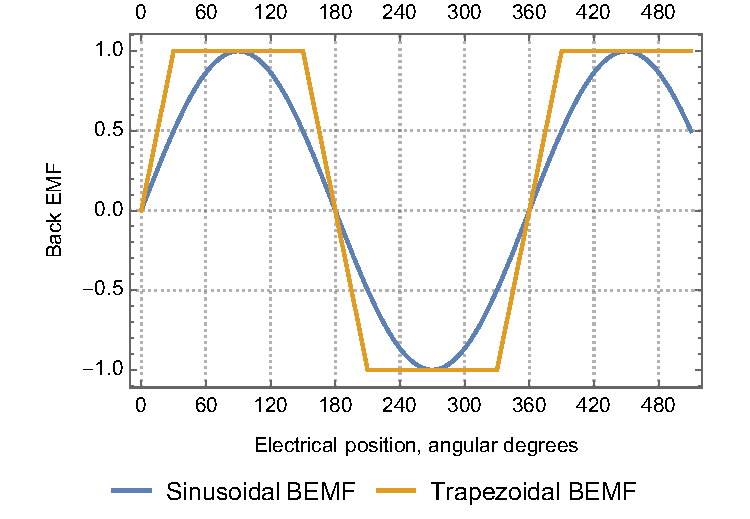
\includegraphics[width=0.6\textwidth]{bemf_trapezoidal_vs_sinusoidal}
	\caption{Difference between trapezoidal and sinusoidal BEMF.
	\label{bemf_trapezoidal_vs_sinusoidal}}
\end{figure}

Sapog, being a BLDC drive, drives the motor with trapezoidal modulated voltage.
This produces smooth torque and vibration free operation with BLDC motors,
since it is expected that the flux linkage will be changing in a specific way.

Like any BLDC drive, Sapog can operate with BLAC motors as well, albeit with increased torque ripple.
From the model presented in section \ref{sec:motor_equations} we can predict that the motor
will exhibit periodic variations in the output torque if the form of the voltage modulated by the controller
does not match with the form of the back EMF induced in the motor.
The resulting periodic torque variations that occur in a BLAC motor driven by a BLDC drive
(and, likewise, in a BLDC motor driven with sine modulated voltages) are shown on the figure 
\ref{sine_torque_deviation}.

\begin{figure}[hbt]
    \centering
	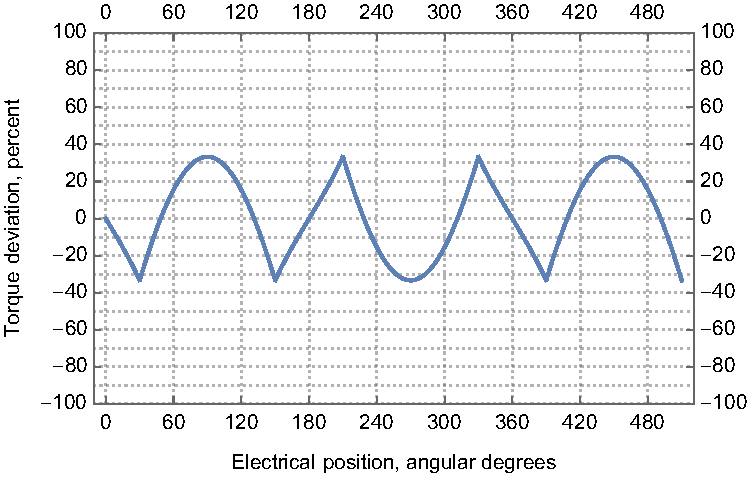
\includegraphics[width=0.6\textwidth]{sine_torque_deviation}
	\caption{Torque ripple caused by mismatching forms of the back EMF and the source voltage.
	\label{sine_torque_deviation}}
\end{figure}

Many applications, however, can tolerate the induced torque ripple and associated vibrations produced
by the motor.

\section{Motor control}

\subsection{Commutation sequence}

\newcommand{\BEMFH}{$\uparrow$}
\newcommand{\BEMFL}{$\downarrow$}

Three phase BLDC drives operate by modulating a specific sequence of voltages on the motor phases
synchronously with the movement of the rotor.
The modulated voltage sequences are shown in the commutation table below
(legend: $+$ -- positive voltage output; $-$ -- negative voltage output;
\BEMFH{} -- the phase is floating, induced BEMF is rising;
\BEMFL{} -- the phase is floating, induced BEMF is falling).

\begin{tabu}{|l c|c c c c c c|}
    \hline
    \rowfont{\bfseries}
    \multicolumn{2}{|c|}{\diagbox{Phase}{Step}}
                                 & 0     & 1     & 2     & 3     & 4     & 5     \\\hline
    \multirow{3}{*}{Forward} & A & $-$   &\BEMFH & $+$   & $+$   &\BEMFL & $-$   \\
                             & B & $+$   & $+$   &\BEMFL & $-$   & $-$   &\BEMFH \\
                             & C &\BEMFL & $-$   & $-$   &\BEMFH & $+$   & $+$   \\\hline
    \multirow{3}{*}{Reverse} & A & $-$   &\BEMFH & $+$   & $+$   &\BEMFL & $-$   \\
                             & B &\BEMFL & $-$   & $-$   &\BEMFH & $+$   & $+$   \\
                             & C & $+$   & $+$   &\BEMFL & $-$   & $-$   &\BEMFH \\\hline
\end{tabu}

The choice between forward and reverse commutation tables affects the direction of rotation of the motor,
and it is specified via the configuration parameter \CfgRef{ctl+dir}.

The rotor position is deduced from the behavior of the induced BEMF on the floating phase.
From figure \ref{bemf_trapezoidal_vs_sinusoidal} we can deduce that when the induced BEMF of the floating
phase crosses the median voltage between the high and the low phase, there is 30 electrical degrees left
before the next commutation step begins.
The controller employs this rule to estimate the time when the next commutation should occur.
The process is demonstrated on the figure \ref{commutation_basics}.
The voltage waveforms shown on the figure were acquired from the phase voltage signal conditioning circuits,
before the ADC inputs, shown on the figure \ref{power_stage_schematic}.

\begin{figure}[hbt]
    \centering
	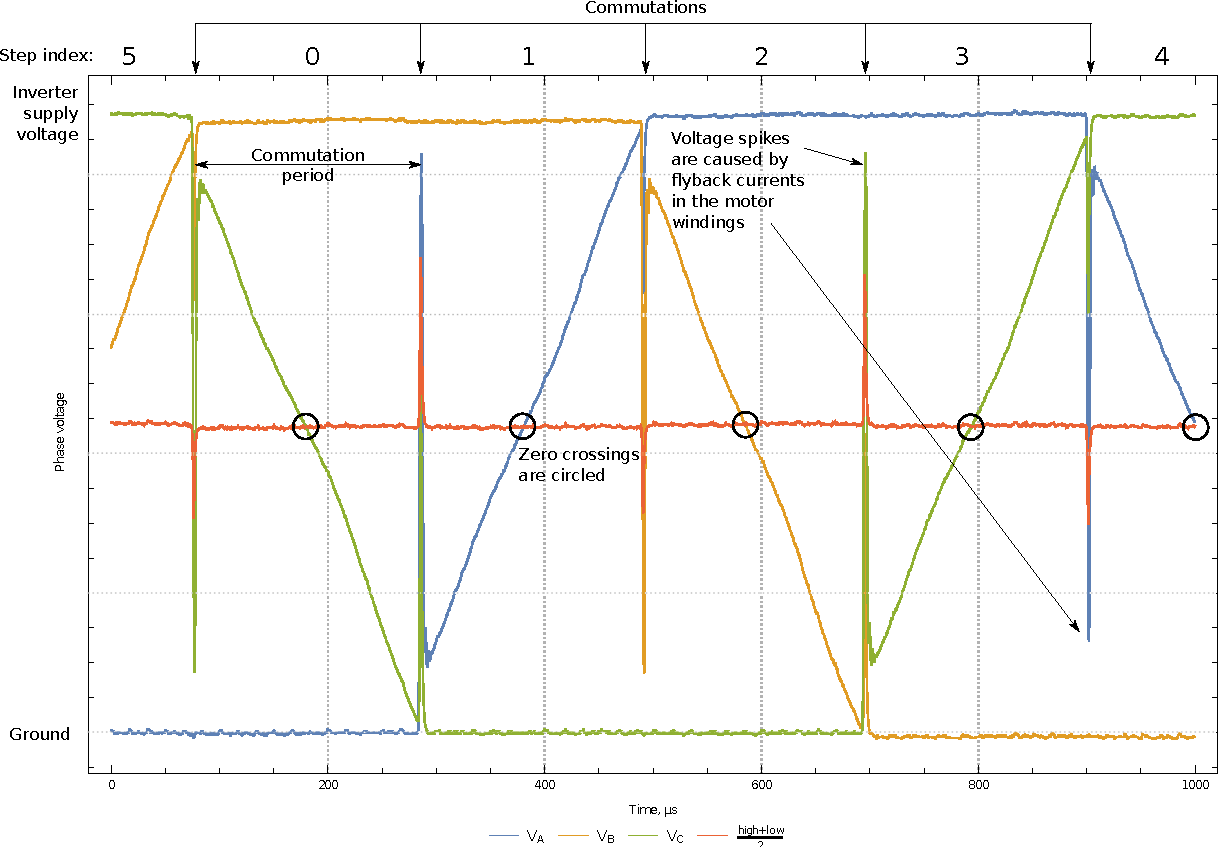
\includegraphics[width=\textwidth]{commutation_basics}
	\caption{Six step commutation sequence observed through phase voltages.
	\label{commutation_basics}}
	PWM modulation is not seen because the shown voltages were acquired while the controller
	was operating at full duty cycle.
\end{figure}

\begin{figure}[hbt]
    \centering
	
\includegraphics[width=\textwidth]{power_stage_schematic}
	\caption{Simplified schematic of the VSI and BEMF feedback circuits that Sapog relies on.
	\label{power_stage_schematic}}
\end{figure}

From the section \ref{sec:motor_equations} we know that the magnitude of the induced BEMF is linearly
dependent on the speed of relative motion between the armature and the rotor magnetic field.
Considering also the fact that the controller relies on the induced BEMF signal for rotor position estimation,
we can predict that the rotor position estimation may be unreliable if the induced BEMF is not sufficiently
strong.
In order to avoid issues at low speed operation, Sapog provides several configuration parameters that
restrict the minimum operating speed, such as the following:

\begin{itemize}
\item \CfgRef{mot+comm+per+max} - maximum commutation period, in microseconds.
The estimated commutation period will be artificially constrained to not exceed this value.
\item \CfgRef{mot+rpm+min} - minimum RPM that can be demanded in RPM governor mode.
If the demanded RPM is lower, the setpoint will be artificially increased.
Reduce this parameter to make the minimum speed lower; increase it to improve stability.
\item \CfgRef{mot+v+min} - minimum source voltage when operating in open loop mode, in volts.
If the demanded duty cycle amounts to a lower source voltage than this, the setpoint will be artificially
increased.
Reduce this parameter to make the minimum speed lower; increase it to improve stability.
\end{itemize}

These parameters may need adjustment to make Sapog compatible with a specific motor.
For example, if the motor cannot keep stable operation at low speed,
the minimum source voltage should be increased,
and/or the maximum commutation period should be made longer.
The minimum voltage limit does not apply to RPM loop mode,
where the minimum speed is governed by the dedicated configuration parameter shown above.

The following equation can be used to convert between commutation period $T_\text{comm}$
and electrical angular velocity $\omega_e$:
\begin{equation}
\omega_e = \frac{\pi}{3 T_\text{comm}}
\end{equation}

\subsection{Source voltage modulation}

Source voltage modulation technique employed by Sapog is a fixed carrier frequency, fixed dead time,
simultaneous 4-quadrant switching PWM modulation.

Four quadrant modulation allows the controller to support active freewheeling and
regenerative braking.

Reviewing different modulation techniques would be outside of the scope of this document.
For more background, the reader is advised to refer to other sources, such as the article
``Influence of PWM Schemes and Commutation Methods for DC and Brushless Motors and Drives''
(Dal Y. Ohm, Richard J. Oleksuk).

The following configuration parameters govern operation of the source voltage modulator:
\begin{itemize}
\item \CfgRef{mot+pwm+hz} - PWM carrier frequency, in hertz.
\item \CfgRef{mot+pwm+dt+ns} - PWM switching dead time, in nanoseconds.
It is not recommended to change this value from the default,
unless there is full understanding of the matter.
\end{itemize}

\subsection{Field weakening}

From section \ref{sec:motor_equations} we know that the maximum speed that a motor can achieve is dependent
on the the load, magnetic flux linkage, and the source voltage.
Reduction of the magnetic flux linkage decreases the induced BEMF, which allows the rotor reach higher speed,
given constant source voltage and load.

The controller can alter the commutation sequence in a specific way, causing the rotating magnetic field
created by the stator to interact with the magnetic field of the rotor in a way that reduces the magnetic
field linkage, effectively increasing the maximum speed of the rotor, reducing the output torque,
while keeping the maximum mechanical power output constant.
Note that since part of the energy is expended on suppression of the magnetic fields induced by the rotor,
the overall efficiency of the drive decreases with higher field weakening.

This technique is known as \emph{field weakening}, and it is implemented by means of adjustment of the 
commutation sequence, shortening the time interval from the zero crossing point to the moment when the next
commutation step begins.
In the context of BLDC drives this specific approach is also known as \emph{commutation advancing}.

Sapog defines commutation advance angle in electrical angular degrees of rotor position,
and it can vary from 0\degree{} to 29\degree{}, inclusively, where 0\degree{} corresponds to no advance,
and 29\degree{} corresponds to the maximum advance angle.
The practical effects imposed on the drive are summarized in the following table.

\begin{ZubaxCompactTable}{|c|c c c c|}
    Advance angle & Flux linkage & Maximum torque & Maximum speed & Drive efficiency \\
    Low           & High         & High           & Low           & High             \\
    High          & Low          & Low            & High          & Low              \\
\end{ZubaxCompactTable}

Sapog can modulate a fixed advance angle, or it can be defined as a function of speed.
The latter is especially useful, since high field weakening at low speeds does not make practical sense,
and serves only to reduce the drive efficiency with no apparent benefit to the application.
Additionally, high field weakening may be responsible for stability issues at low operating speeds,
because it effectively reduces the magnitude of the BEMF induced in the motor.

The field weakening feature is configured with the help of the following configuration parameters:

\begin{itemize}
\item \CfgRef{mot+tim+adv+max} - maximum commutation advance angle, in electrical rotor position degrees.
\item \CfgRef{mot+tim+adv+min} - minimum commutation advance angle, same units.
\item \CfgRef{mot+tim+cp+min} - when the current commutation period is longer than this value,
the minimum advance angle will be used. The units are microseconds.
\item \CfgRef{mot+tim+cp+max} - when the current commutation period is shorter than this value,
the maximum advance angle will be used. Same units.
\end{itemize}

When the current commutation period is between \verb|mot_tim_cp_max| and \verb|mot_tim_cp_min|,
the advance angle will be proportionally linearly interpolated between
\verb|mot_tim_adv_min| and \verb|mot_tim_adv_max|.
The interpolation logic is demonstrated on the figure \ref{timing_advance_interpolation_plot}.

\begin{figure}[hbt]
    \centering
	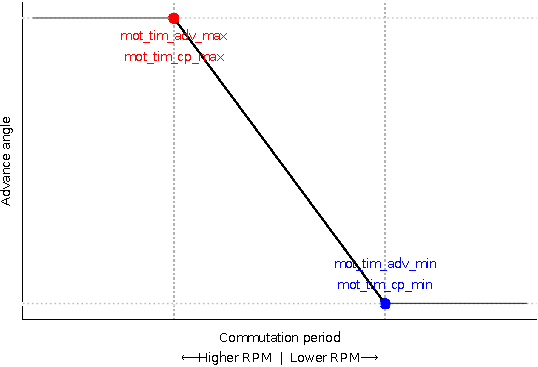
\includegraphics[width=0.7\textwidth]{timing_advance_interpolation_plot}
	\caption{Timing advance interpolation logic.
	\label{timing_advance_interpolation_plot}}
\end{figure}

Sample phase voltage waveforms acquired while the controller was operating under high field
weakening settings are shown on the figure \ref{phase_voltages_at_high_advance_angle}.

\begin{figure}[hbtp]
    \centering
	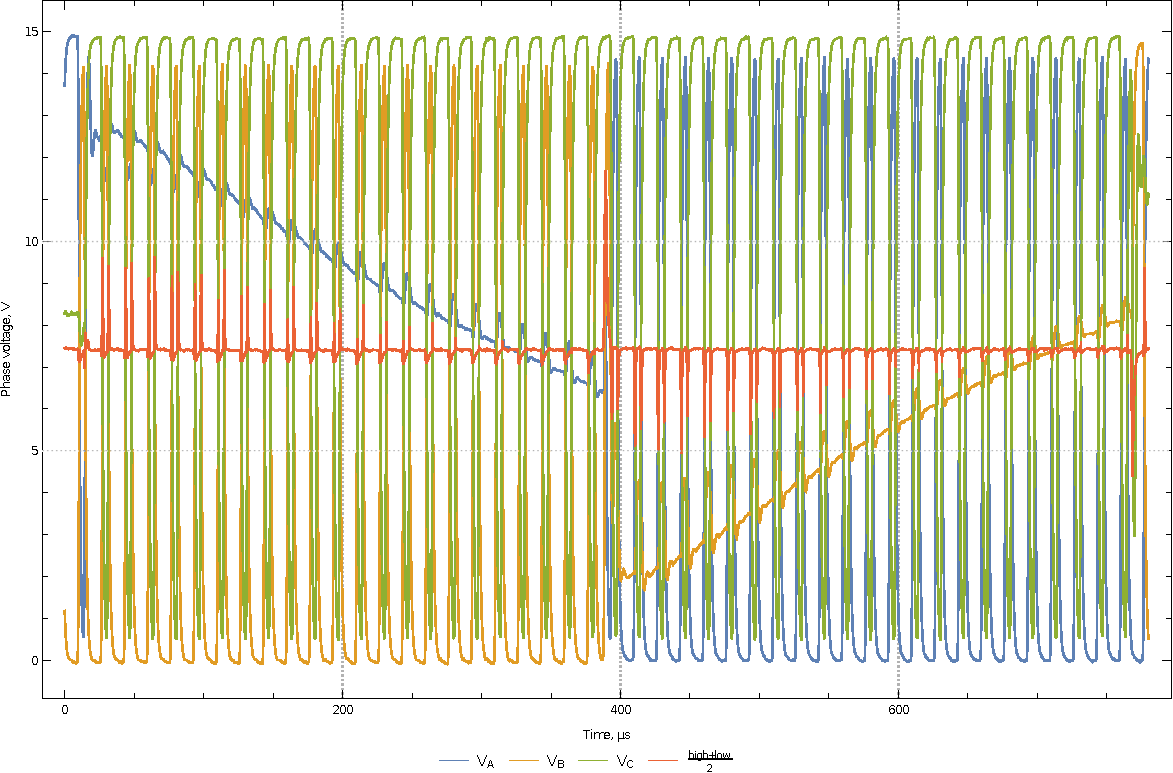
\includegraphics[width=\textwidth]{phase_voltages_at_high_advance_angle}
	\caption{Commutation sequence at high advance angle settings.
	\label{phase_voltages_at_high_advance_angle}}
	It can be seen that the next commutation begins shortly after the induced BEMF
	crosses the neutral voltage.
\end{figure}

\subsubsection{Freewheeling considerations}

Upon careful review of the field weakening effect it might become obvious that it poses certain danger
when the motor is operating at a high speed.

According to the explanations above, as long as the field weakening is active,
the controller actively suppresses the excessive flux of the permanent magnets in the rotor.
This suppression allows the controller to lower the induced BEMF, and, therefore,
extend the operating speed upwards, while keeping the source voltage constant.

Consider what happens when the inverter (or the controller as a whole) is turned off while the
motor was running with the rotor field weakened.
As the controller ceases to suppress the field, the flux linkage of the motor returns to nominal,
which, given that the speed is sufficiently high, may significantly exceed the inverter supply
voltage $V_\text{inv}$, possibly causing damage to the controller, the power supply, the motor, etc.

\subsection{Rotor state observer}

\subsubsection{BEMF processing}

As mentioned previously, Sapog deduces the current position of the rotor by tracking the induced BEMF
on the floating phase.
Which phase is floating and the direction in which BEMF is changing is dependent on the current electrical
angle of the rotor.

Measurement of the induced BEMF is done by the ADC, which is connected to the motor phases via
resistive voltage dividers which reduce the dynamic range of the motor phase voltages into a narrower
dynamic range acceptable by the ADC,
and a buffer capacitor that provides fast recharge of the sample-and-hold capacitor of the ADC,
and suppresses high frequency noise.
The resulting simplified schematic can be seen on the figure \ref{power_stage_schematic}.

BEMF measurements are sensitive to noise. In order to avoid interference with the noise generated
by the VSI, the controller synchronizes BEMF sampling with PWM switching.
However, the timing resolution provided by the resulting sampling pattern is insufficient for robust
rotor state estimation because of the sampling period restrictions imposed by the
PWM carrier frequency.

In order to work around this limitation, Sapog collects a number of samples, and,
knowing that the shape of the BEMF induced by the floating phase of a BLDC motor is linear,
solves a linear regression problem on the collected samples, effectively recovering the most likely
shape of the BEMF signal.
The resulting approximation is very robust and resilient to noise.

The principle is illustrated on the figure \ref{phase_voltage_sampling}.

\begin{figure}[hbtp]
    \centering
	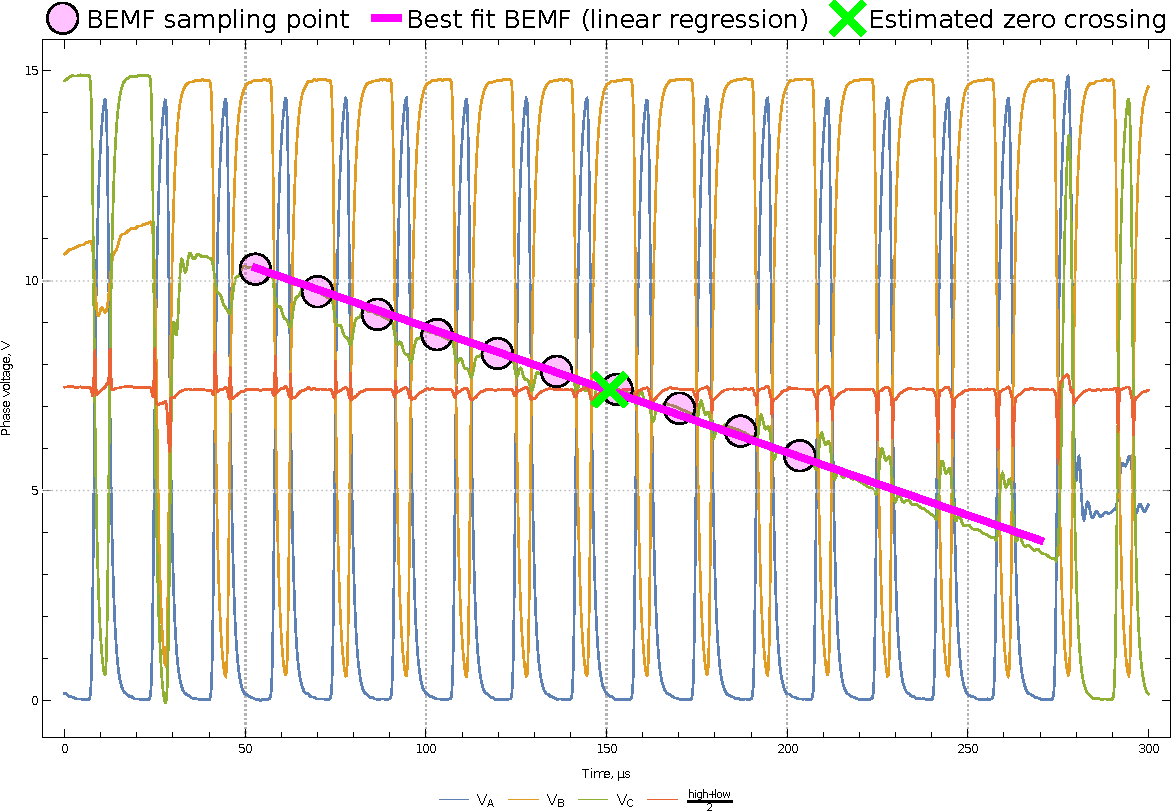
\includegraphics[width=\textwidth]{phase_voltage_sampling}
	\caption{BEMF sampling and PWM modulation.
	\label{phase_voltage_sampling}}
\end{figure}

The number of BEMF samples $N_\text{samples}$ included in the linear regression is defined by
the configuration parameter \CfgRef{mot+bemf+win+den} (dimensionless) as follows:
\begin{equation}
N_\text{samples} =
\frac{T_{\text{comm}} F_{\text{pwm}}}{\frac{\alpha\cdot{}\Pi_\text{bemfwinden}}{15} + \Pi_\text{bemfwinden}} + 2
\end{equation}
where $T_{\text{comm}}$ is the current commutation period,
$\Pi_\text{bemfwinden}$ is the value of the configuration parameter,
$\alpha$ is the current commutation advance angle in electrical rotor position degrees,
and $F_{\text{pwm}}$ is the PWM carrier frequency.

An attentive reader might point out that the assumption of linear BEMF that the described method rests
upon does not hold for BLAC motors, since the induced BEMF of a floating phase will be sinusoidal rather
than linear.
While the objection is correct, this deviation does not pose a significant problem, since the sinusoidal
BEMF well approximates to linear near the point of zero crossing.
Some issues may arise at very high advance angles, where the controller will be forced to resort to
look-ahead extrapolation, so that the linear regression will be applied to the sample set acquired
at the point where the linear approximation assumption does not hold.
The resulting imprecision, however, should not be of significant practical importance.

\subsubsection{Special cases}

The figure \ref{phase_voltage_sampling_corner_cases} provides a closer look at the challenges
seen by the controller in certain operating modes, which are reviewed below.

\begin{figure}[hbtp]
    \centering
	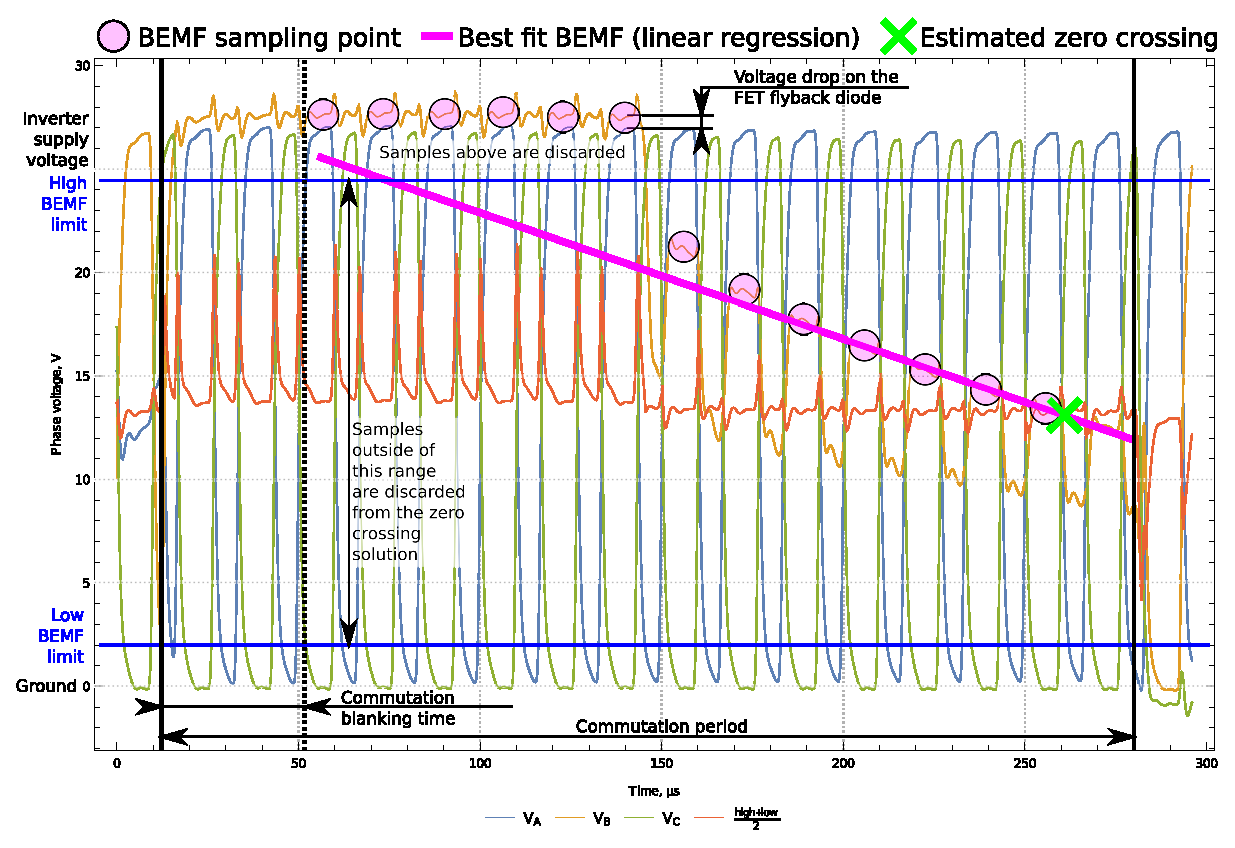
\includegraphics[width=\textwidth]{phase_voltages_braking_high_advance_angle}
	\caption{Corner cases of BEMF sampling.
	\label{phase_voltage_sampling_corner_cases}}
\end{figure}

In certain operating modes the induced BEMF of the floating phase may briefly exceed the
inverter supply voltage $V_\text{inv}$, or fall below the ground level,
causing voltage drop on either the high-side or low-side flyback diodes, respectively.
BEMF samples acquired at this time are not representative of the true form of the signal,
because the signal is altered by external factors;
and therefore, such samples cannot be used for the linear regression.
Sapog uses a simple heuristic that allows it to detect when the sampled signal is subjected to
altering and discard the affected samples.
The heuristic checks whether the sampled voltage falls into a specified range near the neutral voltage,
and discards the sample if it doesn't.

Additionally, samples acquired shortly after commutation may be subjected to transient distortions.
Sapog works around that by imposing a fixed \emph{blanking time} after a commutation, during which
BEMF sampling is not performed.

The following configuration parameters are relevant to the reviewed aspects:

\begin{itemize}
\item \CfgRef{mot+bemf+range} - the voltage range around neutral,
in percent of the inverter supply voltage $V_\text{inv}$, where the BEMF samples
will be considered valid and accepted into the solution.
\item \CfgRef{mot+blank+usec} - duration of the blanking time after the commutation, in microseconds.
\item \CfgRef{mot+spup+blnk+pm} - minimum blanking time during spin-up, permill of the commutation period.
This parameter is reviewed in more detail in a dedicated section.
\end{itemize}

Additional difficulties are posed by operation at very high power levels,
and/or when the controlled motor exhibits high inductance of the windings.
Under these conditions, the motor windings tend to accumulate significant energy during the duration
of the commutation period.
When the current commutation period ends, the winding is released, but the accumulated energy maintains
some current through the winding and the \emph{flyback diode} of one of the transistors until
the energy is dissipated.
This current caused by the energy release from a disconnected inductive network is known as
\emph{flyback current}.
As long as the flyback current is flowing though the winding and the flyback diode,
the induced BEMF is completely suppressed and, therefore,
is unobservable, which does not allow the controller to evaluate the state of the rotor.

\begin{figure}[hbtp]
    \centering
	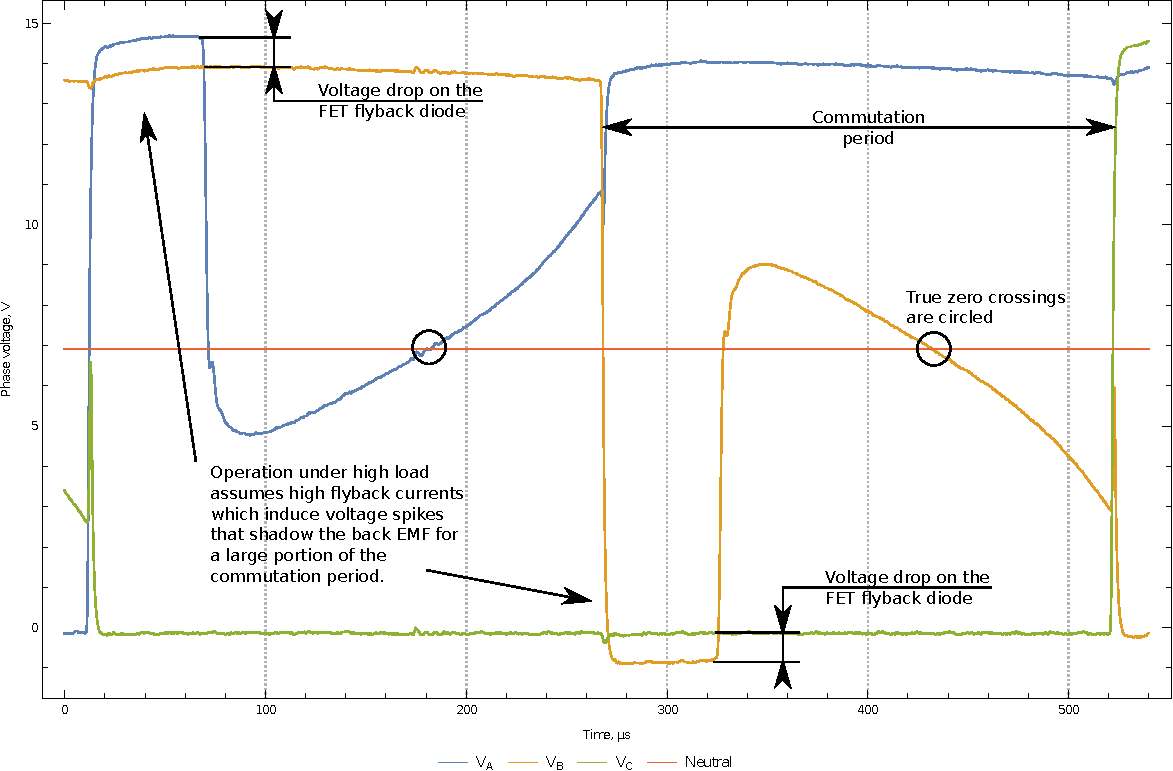
\includegraphics[width=\textwidth]{phase_voltages_at_high_load}
	\caption{Challenges of high power operation.
	\label{phase_voltages_at_high_load}}
\end{figure}

Sapog recognizes this condition and waits for the flyback current to cease.
If the current is still flowing past a certain deadline necessary for the controller to evaluate the
point of zero crossing, Sapog enters a \emph{desaturation mode} in order to bring the system
back into observable state.
In the desaturation mode Sapog turns off the inverter and waits until the next commutation period.
By the time the next commutation period begins, the flyback currents will have ended,
allowing the controller to continue observation of the motor state.

The figure \ref{phase_voltages_at_high_load} shows operation near the point of activation
of the desaturation mode.

\subsubsection{Maximum speed restrictions}

It is easy to see that as the speed increases and the commutation period shortens,
the number of BEMF samples that can be accommodated within the commutation period will be decreasing.
This effect imposes the limit on the maximum achievable speed, and the limit is dependent on the PWM
carrier frequency.

When the drive operates in open loop mode, the controller will limit the maximum duty cycle
when the commutation period reaches dangerously low values.
The limiting is done by means of a simple P-controller,
which begins to override the duty cycle setpoint when it exceeds a certain value.

When the drive operates in RPM control loop mode, the limiting will be performed simply by means of
clipping the RPM setpoint.

The exact thresholds are specified on the figure \ref{pwm_maximum_speed}.

The configuration parameter \CfgRef{mot+pwm+hz} can be used to set the desirable PWM frequency
in hertz.
It is recommended to keep the frequency as low as possible,
as that would facilitate lower switching losses and therefore higher efficiency of the drive.

\begin{figure}[hbt]
    \centering
	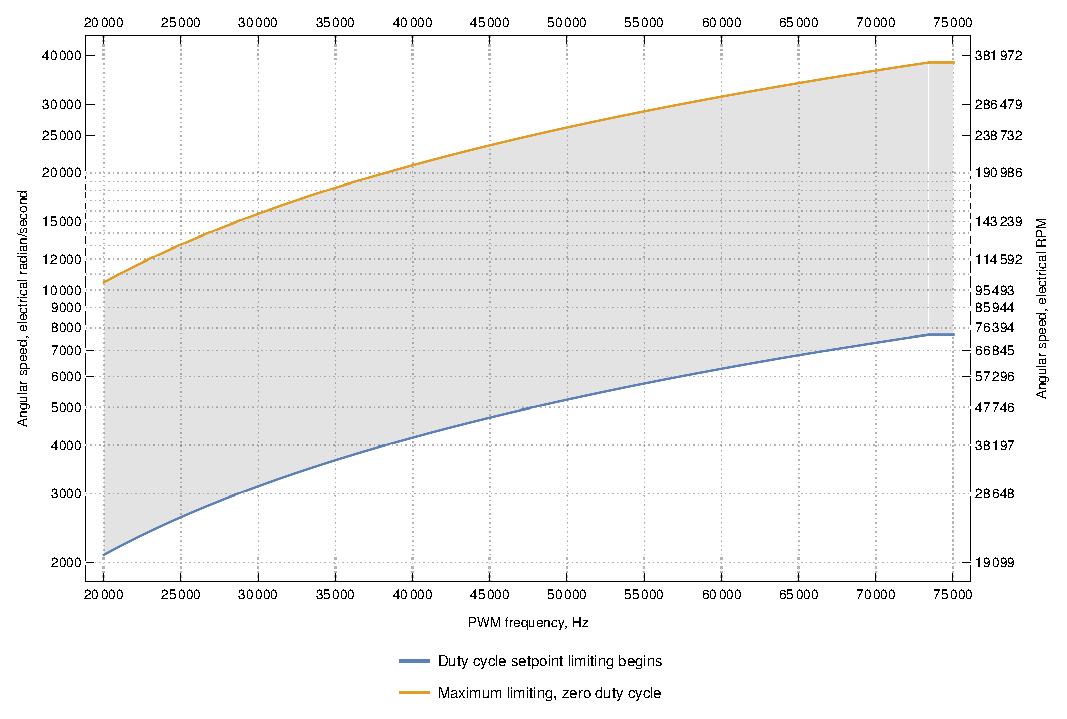
\includegraphics[width=\textwidth]{pwm_maximum_speed}
	\caption{Dependency of the maximum speed on PWM frequency.
	\label{pwm_maximum_speed}}
\end{figure}

\subsubsection{Field weakening restrictions}

The controller requires several microseconds to solve the linear regression problem after the sampling is
finished.
However, operation at very high advance angles requires the controller to perform commutation virtually
immediately after the zero crossing has happened, leaving very little time to perform the computation.
The controller strives to work around this contradiction by trying to robustly extrapolate the shape of the
BEMF signal, predicting the upcoming zero crossing ahead of time.

Despite that, operation at very high speeds may not provide the time necessary to take a sufficient
number of samples and solve the regression problem before the next commutation is due.
In this case, Sapog will silently lower the current advance angle and keep it at as close to the requested
value as the current operating mode permits.

\subsection{Regenerative braking}

During regenerative braking, the source voltage $E_s$ modulated by the controller is lower than the
induced BEMF $E_b$, which causes reverse current flow from the motor into the VSI
and further into the power supply network.
According to the formulas presented in the section \ref{sec:motor_equations},
reversing the current will also reverse the torque, causing the motor to rapidly decelerate.

This process converts the mechanical energy of the motor into electrical energy returned back into the
power supply network.
If the power supply network cannot absorb the recovered energy (e.g. due to its resistance being too high),
the regenerative energy transfer may lead to increase of the supply voltage beyond the safe operating limits.
Typically, the controller hardware is equipped with some protection circuits that activate and dissipate the
excessive energy when $V_\text{inv}$ increases a certain threshold;
however, their energy absorption capabilities are often very  limited.

Generally, batteries are capable of absorbing the regenerated energy during braking without issues.
Problems may arise if the controller is powered from a source that does not permit reverse currents,
such as laboratory power supplies or some types of voltage conversion circuits.

Refer to the documentation provided with your hardware to learn more about the issues
concerning regenerative braking and the excess energy release.

\subsection{Rotor stall detection}

Rotor stall is a condition where the rotor ceases to rotate due to the torque generated by the motor
being lower than the mechanical load on the shaft.
Sapog detects this condition by observing a specific number of failures to find
a valid BEMF zero crossing event.

As explained in one of the earlier sections of this document,
Sapog requires the rotor to move in order to be able to operate normally.
Once the rotor has stalled, Sapog will shut down the VSI and wait for the next setpoint to arrive.
Once the next setpoint has arrived, Sapog will restart the motor normally,
unless the number of consecutive stalls has exceeded a specific limit.

In the latter case, Sapog will lock up and refuse to start the motor again,
until it has received a zero setpoint.
Zero setpoint is treated as a reset command that clears the stall counter and unlocks the controller.

Zero cross failures are counted with the help of a dedicated counter state.
When Sapog fails to find a zero crossing solution,
the failure counter is incremented by one.
When Sapog succeeds to perform six (6) commutations in a row without failures,
the failure counter is reset back to zero.

The following configuration parameters configure the behaviors pertaining to stall detection:

\begin{itemize}
\item \CfgRef{mot+zc+fails+max} - zero crossing detection failure threshold.
If the failure counter exceeds this threshold, the rotor will be considered stalled.
\item \CfgRef{mot+stop+thres} - lock-up threshold.
If the rotor has stalled this number of times in a row,
the controller will lock up until a zero setpoint is received.
\end{itemize}

\subsection{Spin-up}

As has been explained before, Sapog requires the rotor to move in order to be able to operate normally,
because the state estimation methods that work well when the rotor is moving break apart when the rotor is
stationary or nearly so.

From the above follows that a different method of state estimation is needed to start the motor
from standstill, especially so if the shaft is attached to a mechanical/inertial load.

\subsubsection{Algorithm}

When starting the motor, Sapog sets the source voltage $E_s$ to the value specified in the
configuration parameter \CfgRef{mot+v+spinup}, and activates the commutation step at the index 1.
Having done so, Sapog begins to wait for the zero crossing detector to report that it is time to
begin the next commutation period; until the amount of time specified by the configuration parameter
\CfgRef{mot+spup+st+cp} expires, whichever happens first.
Afterwards, Sapog switches to the next commutation step, and the process repeats again.

While in spin-up mode, Sapog will slowly increase the voltage from the initial value specified
by \CfgRef{mot+v+spinup} until the minimal operating voltage \CfgRef{mot+v+min} is reached.
The duration of the spin-up voltage ramp is specified by the parameter \CfgRef{mot+spup+vramp+t},
in seconds.
The ramp is graphically illustrated on the image \ref{spinup_voltage_ramp}.

\begin{figure}[hbt]
    \centering
	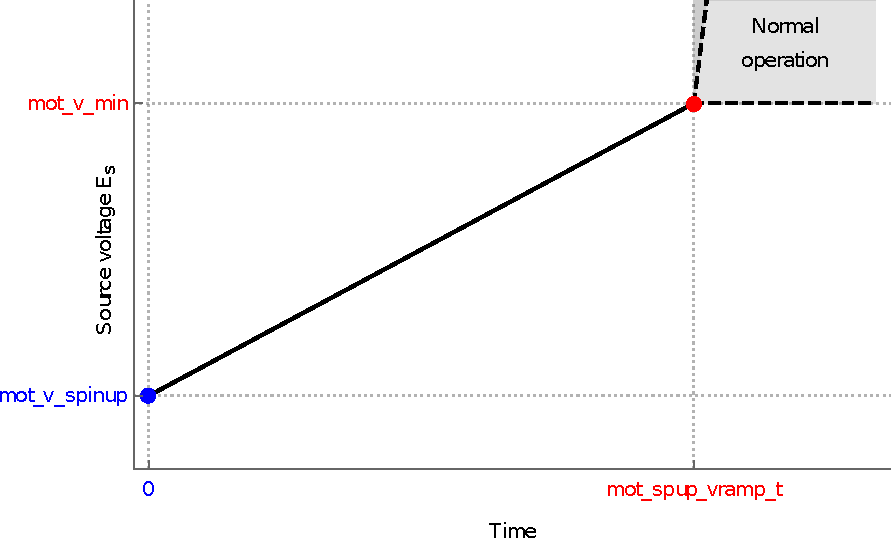
\includegraphics[width=0.7\textwidth]{spinup_voltage_ramp}
	\caption{Voltage ramp during spin-up.
	\label{spinup_voltage_ramp}}
\end{figure}

It should be noted that high initial voltages and/or steep voltage ramps need to be avoided,
because they may lead to severe instabilities in the beginning of the spin-up sequence.
Keep in mind that it is virtually impossible for any synchronous sensorless drive to create stable
torque at low speeds, and especially at standstill.

While spin-up is in progress, Sapog always operates at the zero advance angle
(field weakening disabled) for the reasons explained earlier,
regardless of the configured advance angle settings.

\subsubsection{Spin-up rotor state observer}

The zero crossing detector mentioned above operates in a very different way compared to the
normal rotor state observer used in the normal operating mode.

While operating in spin-up mode, the observable behavior of the induced BEMF may be very erratic,
mainly due to the low magnitude of the signal and irregular rotation of the rotor caused by
imprecise synchronization of the modulated field with the field of the rotor.
In order to combat these difficulties, Sapog employs a different kind of observer, which provides
more robust operation at low speeds.

Immediately after commutation Sapog inserts a blanking delay $T_\text{blank}$
defined by the following equation:
\begin{equation}
T_{\text{blank}}=
\max \left(\frac{\Pi_{\text{blankusec}}}{10^6},
\frac{\Pi_{\text{spupblnkpm}} T_{\text{comm}}}{1000}\right)
\end{equation}
where $\Pi_{\text{spupblnkpm}}$ is the value of the configuration parameter \CfgRef{mot+spup+blnk+pm}
(permill of the commutation period),
$T_{\text{comm}}$ is the duration of the last commutation period,
$\Pi_{\text{blankusec}}$ is the value of the configuration parameter \CfgRef{mot+blank+usec}
(in microseconds).

Upon expiration of the blanking delay, Sapog watches the BEMF waiting for the flyback current to cease.
Afterwards, Sapog starts to integrate the sampled BEMF voltages relative to the neutral voltage.
Once the integrated voltage changes the sign, Sapog switches to the next commutation period.
A more formal definition of the commutation condition is shown below:
\begin{equation}
\begin{aligned}
&\sum_{n} E_{s_n} - E_{\text{neutral}_n} > 0 \qquad\text{for rising BEMF}\\
&\sum_{n} E_{s_n} - E_{\text{neutral}_n} < 0 \qquad\text{for falling BEMF}
\end{aligned}
\end{equation}

The principle is illustrated on the oscillogram \ref{spinup_phase_voltages}.

\begin{figure}[hbt]
    \centering
	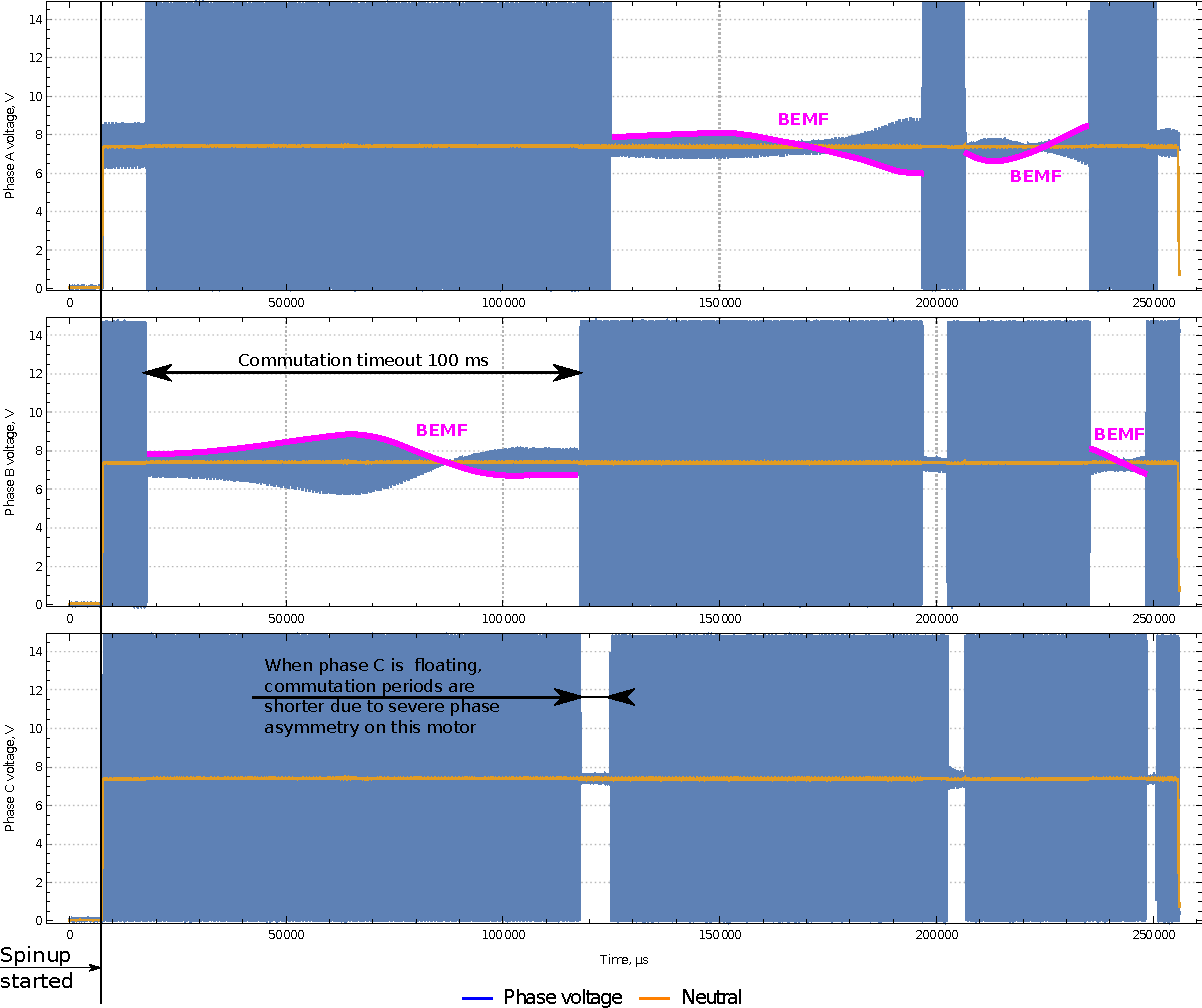
\includegraphics[width=\textwidth]{spinup_phase_voltages}
	\caption{Spin-up sequence with a highly inertial load.
	\label{spinup_phase_voltages}}
\end{figure}

\subsubsection{Termination conditions}

Spin-up will be considered finished once the maximum commutation period defined by the parameter
\CfgRef{mot+comm+per+max} \emph{and} the minimum voltage \CfgRef{mot+v+min} are reached.
Should the target commutation period be reached earlier than the voltage ramp comes to the final
voltage level, the controller will significantly accelerate the ramp in order to converge to
the minimum operating voltage faster.
Once spin-up is finished, the controller will abandon the spin-up mode and switch into normal mode.

If the target commutation period could not be reached in the amount of time specified by
the parameter \CfgRef{mot+spup+to+ms}, in milliseconds, the controller will abort spin-up,
shut down the VSI and register it as a regular rotor stall event.

\subsubsection{Spin-up from non-stationary state}

Sapog assumes that the rotor is (nearly) stationary in the beginning of the spin-up process.
If this assumption is violated, there may be brief transient processes involving abnormal currents,
high vibrations and high EMI.

The transient currents can be either forward or regenerative, depending on whether the desired
and the actual directions of rotation match, and whether the initial guess of the current
commutation step was correct.

Typically Sapog can establish adequate synchronization in a few steps.
If the rotor was rotating in the same direction but at a higher speed,
it will be rapidly decelerated until the speed defined by the load and the source voltage is
reached.
If it is expected that the motor will be frequently started from non-stationary state,
it is recommended to either shorten the initial voltage ramp, or increase the initial
spin-up voltage, in order to reduce the stresses caused by initial braking.

\subsubsection{Configuration parameters}

This section summarizes information about the configuration parameters pertaining to the spin-up mode.
Read the preceding sections for a more detailed review.

\begin{itemize}
\item \CfgRef{mot+spup+blnk+pm} - duration of the extended blanking time during spin-up in permill
(i.e. one-thousands; $10\text{\space{}permill} = 1\% $) of the current commutation period.
\item \CfgRef{mot+spup+to+ms} - overall spin-up timeout, in milliseconds.
If spin-up could not be completed in this amount of time, the rotor will be considered stalled.
\item \CfgRef{mot+spup+st+cp} - maximum commutation period for spin-up mode, in microseconds.
This is also the initial commutation period.
\item \CfgRef{mot+spup+vramp+t} - duration of the initial voltage ramp, in seconds.
\item \CfgRef{mot+v+spinup} - initial source voltage $E_s$ in the beginning of the voltage ramp, in volts.
\end{itemize}

\subsection{Open loop operation}\label{sec:open_loop}

While operating in the open loop mode, Sapog accepts setpoints in the range from 0\% to 100\%,
and treats that as the fraction of the inverter supply voltage $V_\text{inv}$ to
deliver to the motor $E_s$:
\begin{equation}
E_s = V_\text{inv}\cdot{}\mathrm{ramp}\left(\mathrm{limit}\left(S_\text{DC}\right)\right)
\qquad\text{for open loop mode}, S_\text{DC} \in \left(0, 1\right]
\end{equation}
where $S_\text{DC}$ is the setpoint (DC stands for \emph{duty cycle}),
$\mathrm{ramp}$ is the setpoint ramp function,
and $\mathrm{limit}$ is the speed limiting P-controller, reviewed below.

The ramp function replaces abrupt changes in the setpoint with gradual changes.
Abrupt changes that are small enough to not be a hazard to stability of the drive are
accepted by the controller directly, bypassing the ramp.
The following configuration parameters govern the open loop setpoint ramp:

\begin{itemize}
\item \CfgRef{mot+dc+slope} - the slope of the setpoint ramp, in full ranges per second.
For example, the value of 1 allows the controller to sweep the setpoint from 0\% to 100\% in 1 second.
The value of 10 allows the controller to sweep the setpoint from 0\% to 100\% in 0.1 seconds.
\item \CfgRef{mot+dc+accel} - the maximum change in setpoint that will be propagated directly,
bypassing the ramp.
For example, the value of 0.1 allows the controller to apply step changes up to 10\% large directly.
\end{itemize}

Increase the parameters (either one or both) to improve the response characteristics of the drive.
Reduce them if rapid setpoint changes cause stability issues.

Note that the minimum acceptable setpoint is constrained by the minimum duty cycle deduced from
the parameter \CfgRef{mot+v+min}.
If the setpoint falls into $\left(0, S_{\text{DC}_\text{min}}\right]$,
where $S_{\text{DC}_\text{min}}$ is the minimum
duty cycle deduced from the parameter \CfgRef{mot+v+min},
it will be silently overridden to $S_{\text{DC}_\text{min}}$.

The maximum acceptable setpoint will be automatically limited by means of a simple
P-controller\footnote{Proportional controller, i.e. only P term of a PID controller is implemented.}
if the motor approaches the maximum operating speed permitted by the
current PWM carrier frequency, as shown on the figure \ref{pwm_maximum_speed}.

A zero setpoint is treated as the command to stop the motor.
While the motor is stopped, the VSI is disabled, allowing the shaft to rotate freely.

\subsection{RPM control loop}

When operating in the RPM control mode, also known as RPM governor mode,
Sapog will try to maintain a specified mechanical speed.
Speed control is implemented by means of a parallel PID controller
that takes the current mechanical RPM as input and
produces the duty cycle setpoint at the output.

The nominal update rate of the PID controller $T_{\text{RPMPID}}$ is defined as follows:
\begin{equation}\label{eq:rpm_pid_control_loop_period}
T_{\text{RPMPID}} \approx \max \left(10^{-3},T_{\text{comm}}\right)
\end{equation}
where $T_\text{comm}$ is the current commutation period.
Update of the RPM control loop is not a hard real time process, and the software is allowed to
deviate.

RPM control loop relies on the duty cycle slope control function defined in the section \ref{sec:open_loop},
so the related configuration parameters are still applicable.
The speed limiting P-controller that is used in the open loop mode, however,
is entirely bypassed in RPM mode.
The maximum supported speed is dependent on the PWM carrier frequency;
see the figure \ref{pwm_maximum_speed} for details.
Equation \ref{eq:speed_electrical_mechanical} defines the relation between electrical
and mechanical angular rates.

If the commanded setpoint is lower than the value specified by the parameter \mbox{\CfgRef{mot+rpm+min},}
the actual setpoint will be silently increased to match this value.
A zero setpoint is treated as the command to stop the motor.
While the motor is stopped, the VSI is disabled, allowing the shaft to rotate freely.

The RPM PID controller does not wind up the integral term if the output is constrained by external factors,
such as:
\begin{itemize}
\item Duty cycle ramp.
\item Current limiting controller.
\item Maximum RPM limit.
\end{itemize}

The configuration parameters listed below govern operation of the RPM control loop.
The symbol $\text{DC}$ refers to the duty cycle unit ranging in $\left[-1, 1\right]$,
where negative values correspond to negative inverter source voltage $E_s$.

\begin{itemize}
\item \CfgRef{mot+num+poles} - the number of magnetic poles on the rotor, always even, always $\geq 2$.
This parameter is needed for the controller to convert the electrical speed $\text{RPM}_e$
into mechanical $\text{RPM}_m$.
\item \CfgRef{rpmctl+p} - proportional term of the RPM PID controller,
in $\frac{\text{DC}}{\text{RPM}_m}$.
\item \CfgRef{rpmctl+i} - integral term of the RPM PID controller,
in $\frac{\text{DC}}{\text{second}\cdot{}\text{RPM}_m}$.
\item \CfgRef{rpmctl+d} - derivative term of the RPM PID controller,
in $\frac{\text{second}\cdot{}\text{DC}}{\text{RPM}_m}$.
\item \CfgRef{mot+rpm+min} - minimum mechanical RPM at which stable operation is guaranteed.
\end{itemize}

The overall RPM control loop output for time step $n$ can be approximated with the following equations:
\begin{equation}
e(n) = \omega_{m_{n}} - S_{\omega_{m_{n}}}
\end{equation}
\begin{equation}
E_{s_n} = V_{\text{inv}_n}\cdot\mathrm{ramp}
\left[
\underbrace{\frac{e\left(n\right) - e\left(n-1\right)}{T_{\text{RPMPID}}} \Pi_{\text{rpmctld}}}_\text{derivative} +
\mathrm{clamp}\left(\underbrace{\sum_{i=0}^n e\left(i\right) \Pi_{\text{rpmctli}}}_\text{integral}\right) +
\underbrace{e\left(n\right) \Pi_{\text{rpmctlp}}}_\text{proportional}
\right]
\end{equation}
where:
\begin{itemize}
\item $\mathrm{ramp}$ - slope control function defined in the section \ref{sec:open_loop}.
\item $\mathrm{clamp}$ - integrator wind-up control function described in this section.
\item $\omega_{m}$ - current speed, in mechanical RPM.
\item $S_{\omega_{m}}$ - target speed setpoint, in mechanical RPM.
\item $T_{\text{RPMPID}}$ - instant control loop update period.
See equation \ref{eq:rpm_pid_control_loop_period}.
\item $\Pi_{\text{rpmctlp}}$ - proportional term of the PID controller.
\item $\Pi_{\text{rpmctli}}$ - integral term of the PID controller.
\item $\Pi_{\text{rpmctld}}$ - derivative term of the PID controller.
\end{itemize}

\subsection{Current measurement}



\section{Self diagnostics}



\chapter{Configuration parameters}

\CfgDef{esc+index}
\CfgDef{cmd+ttl+ms}
\CfgDef{cmd+start+dc}
\CfgDef{uavcan+node+id}
\CfgDef{light+index}
\CfgDef{pwm+max+usec}
\CfgDef{pwm+min+usec}
\CfgDef{pwm+enable}
\CfgDef{enum+max+step}
\CfgDef{enum+steps}
\CfgDef{enum+bemf}
\CfgDef{mot+pwm+dt+ns}
\CfgDef{mot+pwm+hz}
\CfgDef{mot+spup+blnk+pm}
\CfgDef{mot+spup+to+ms}
\CfgDef{mot+spup+st+cp}
\CfgDef{mot+comm+per+max}
\CfgDef{mot+zc+fails+max}
\CfgDef{mot+bemf+range}
\CfgDef{mot+bemf+win+den}
\CfgDef{mot+blank+usec}
\CfgDef{mot+tim+cp+min}
\CfgDef{mot+tim+cp+max}
\CfgDef{mot+tim+adv+max}
\CfgDef{mot+tim+adv+min}
\CfgDef{mot+i+shunt+mr}
\CfgDef{rpmctl+i}
\CfgDef{rpmctl+d}
\CfgDef{rpmctl+p}
\CfgDef{mot+stop+thres}
\CfgDef{mot+lpf+freq}
\CfgDef{mot+i+max+p}
\CfgDef{mot+i+max}
\CfgDef{mot+rpm+min}
\CfgDef{ctl+dir}
\CfgDef{mot+num+poles}
\CfgDef{mot+dc+slope}
\CfgDef{mot+dc+accel}
\CfgDef{mot+spup+vramp+t}
\CfgDef{mot+v+spinup}
\CfgDef{mot+v+min}

\end{document}
